\documentclass[12 pt,a4paper,fleqn]{article}
\usepackage[brazilian]{babel}
\usepackage[utf8]{inputenc}
\usepackage[T1]{fontenc}
\usepackage{amsfonts}
\usepackage{amsmath}
\usepackage{amssymb}
\usepackage{graphicx}
\usepackage{hyperref}
\usepackage[all]{xy}
\usepackage[left=2cm, right=2cm, bottom=3cm, top=2cm]{geometry}
\usepackage{rotating}
\usepackage{textcomp}
\usepackage{flowchart}
\usepackage{float}


\begin{document}
\begin{center}
	\Large{\textbf{SIMULAÇÃO ARTIFICIAL DE EVOLUÇÃO NEURONAL}}
\end{center}\bigskip\bigskip
	
\section{Introdução}
	Queremos simular um cérebro digital, mas por uma via diferente das redes neurais artificiais conhecidas. Em vez de disso, teremos uma malha 3D de neurônios que poderão se conectar e se comunicar de maneiras semelhantes às que temos na natureza. Essas estruturas são determinadas geneticamente. Através da simulação de agentes/organismos digitais em certos ambientes, suas estruturas neuronais irão evoluir com algoritmos genéticos. Com isso, esperamos obter estruturas mais orgânicas e, portanto, mais próximas de uma inteligência artificial geral.
	
\section{Estrutura do cérebro}
	Cada cérebro é um tensor $a \times b \times c$, com $a, b, c \geq 2$ naturais. Cada nó deste tensor é um neurônio do cérebro. Alguns destes neurônios são responsáveis por receber sinais de input, outros são responsáveis por retornar os outputs, e os outros recebem e enviam sinais entre si. Há conexões entre os neurônios, mas não necessariamente todos estão conectados com todos, nem há a noção de "camadas"\ ("layers") como temos em redes neurais tradicionalmente. 
	
	Por haver conexão entre certos nós, podemos interpretar a estrutura cerebral não como um tensor, mas como um gráfo parcialmente conectado, em que cada nó é identificado por um tupla de 3 números.
	
	\begin{figure}[H]
		\centering
		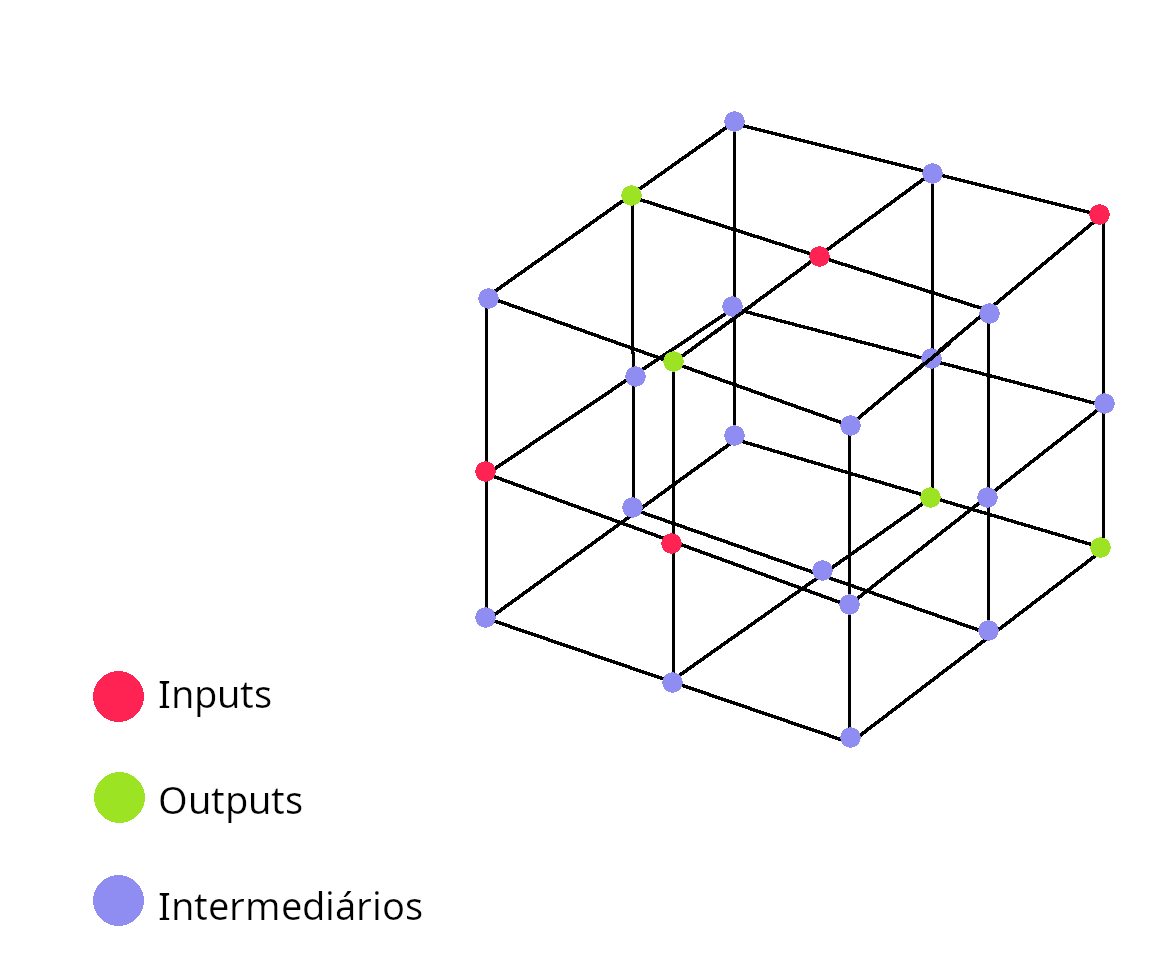
\includegraphics[scale=1]{tensor} 
		\caption{\footnotesize{Exemplo de estrutura de um possível cérebro. Note que os neurônios de inputs e outputs podem estar em qualquer lugar. a posição deles é definida geneticamente e não existe nenhum restrição sobre isso.}}
	\end{figure}	
	
\section{Inputs}
	Um input pode ser a temperatura do ambiente, uma percepção de força aplicada sobre determinada parte do corpo do agente, a velocidade do agente em alguma direção, etc. Basicamente qualquer percepção sensorial externa ou interna pode ser um input para o agente. Cada input é direcionada para um, e apenas um, neurônio deste agente. Se ter múltiplos neurônios recebendo o mesmo input é algo vantajoso, a própria evolução natural irá "descobrir"\ um cérebro onde esse único neurônio de input envia o sinal inalterado do input para outros neurônios. Com isso, o mesmo resultado é obtido sem intervenção forçada no design\footnote{É bom deixar claro logo que a proposta deste trabalho é obter estruturas cerebrais com o mínimo de intervenção possível. Se alguma certa estrutura for melhor que outras, ela deverá ser "descoberta"\ naturalmente em vez de imposta na metodologia.} do cérebro. 
	
\section{Outputs}
	Os outputs são as possíveis ações que um agente pode executar. Todas estas ações devem ser definidas previamente. Similarmente aos inputs, cada output do agente está associado a um, e apenas um, neurônio. Cada um destes neurônios possui um threshold, que é um dos valores $ \{0.2,\ 0.4,\ 0.6,\ 0.8\}$. Seja $x$ o sinal recebido pelo neurônio de output. Se $\sigma(x) = 1 - e^{-\frac{x}{\kappa}}$ é maior que este threshold, então o agente irá executar a ação associada, em que $1 \leq \kappa \leq 4$ é uma constante definida geneticamente e associada ao cérebro.
	
\section{Envio de sinais}
	Cada neurônio possui uma vizinhança de neurônios para os quais ele transmite sinais. Essa vizinhança é uma região retangular 3D que é determinada geneticamente. Cada neurônio possui uma região de dimensões próprias, ou seja, a região pode ter um tamanho diferente para cada neurônio. Vale ressaltar que neurônios de output também possuem estas regiões. Então, após este neurônio fazer com o que o agente execute uma ação, ele ainda transmite o sinal para outros neurônios. É como se o cérebro quisesse que mais neurônios fiquem cientes de que a ação foi realizada.
	
	Um input externo pode ser qualquer número real. Ao receber um input $x$, ele é convertido para o sinal $\hat{x} = \sigma(x)$. É assim que um input é recebido pelo neurônio de input. Cada neurônio conectado ao neurônio do input recebe este sinal como $\varepsilon \cdot \sigma(\hat{x})$, em que $\varepsilon$ é a força da conexão entre estes neurônios. Algumas observações se fazem necessárias aqui:
	
	\begin{enumerate}
		\item Só existe uma conexão entre dois neurônios, e ela é direcional. Ou seja, se o neurônio A envia sinais para B, então B não consegue enviar sinais para A. Todas estas conexões são determinadas geneticamente, mas elas podem ser alteradas ao longo da vida do agente. Falaremos mais disso adiante.
		\item A força das conexões começa sendo igual a $1$ para todas as conexões. Ao longo da vida do agente estas forças são atualizadas induvidualmente, podendo aumentar ou diminuir conforme a conexão é muito ou pouco utilizada. 
	\end{enumerate}
	


			
\end{document}